\subsection{La classe Object et ses filles}

Pour rappel, la classe object permet de définir toutes les entités du jeu.
Tout type définit par l'utilisateur hérite de cette classe ou de l'une de ces classes filles.
Elles sont présentées dans le schéma ci-dessous :

\begin{figure}[h]
 \centering
 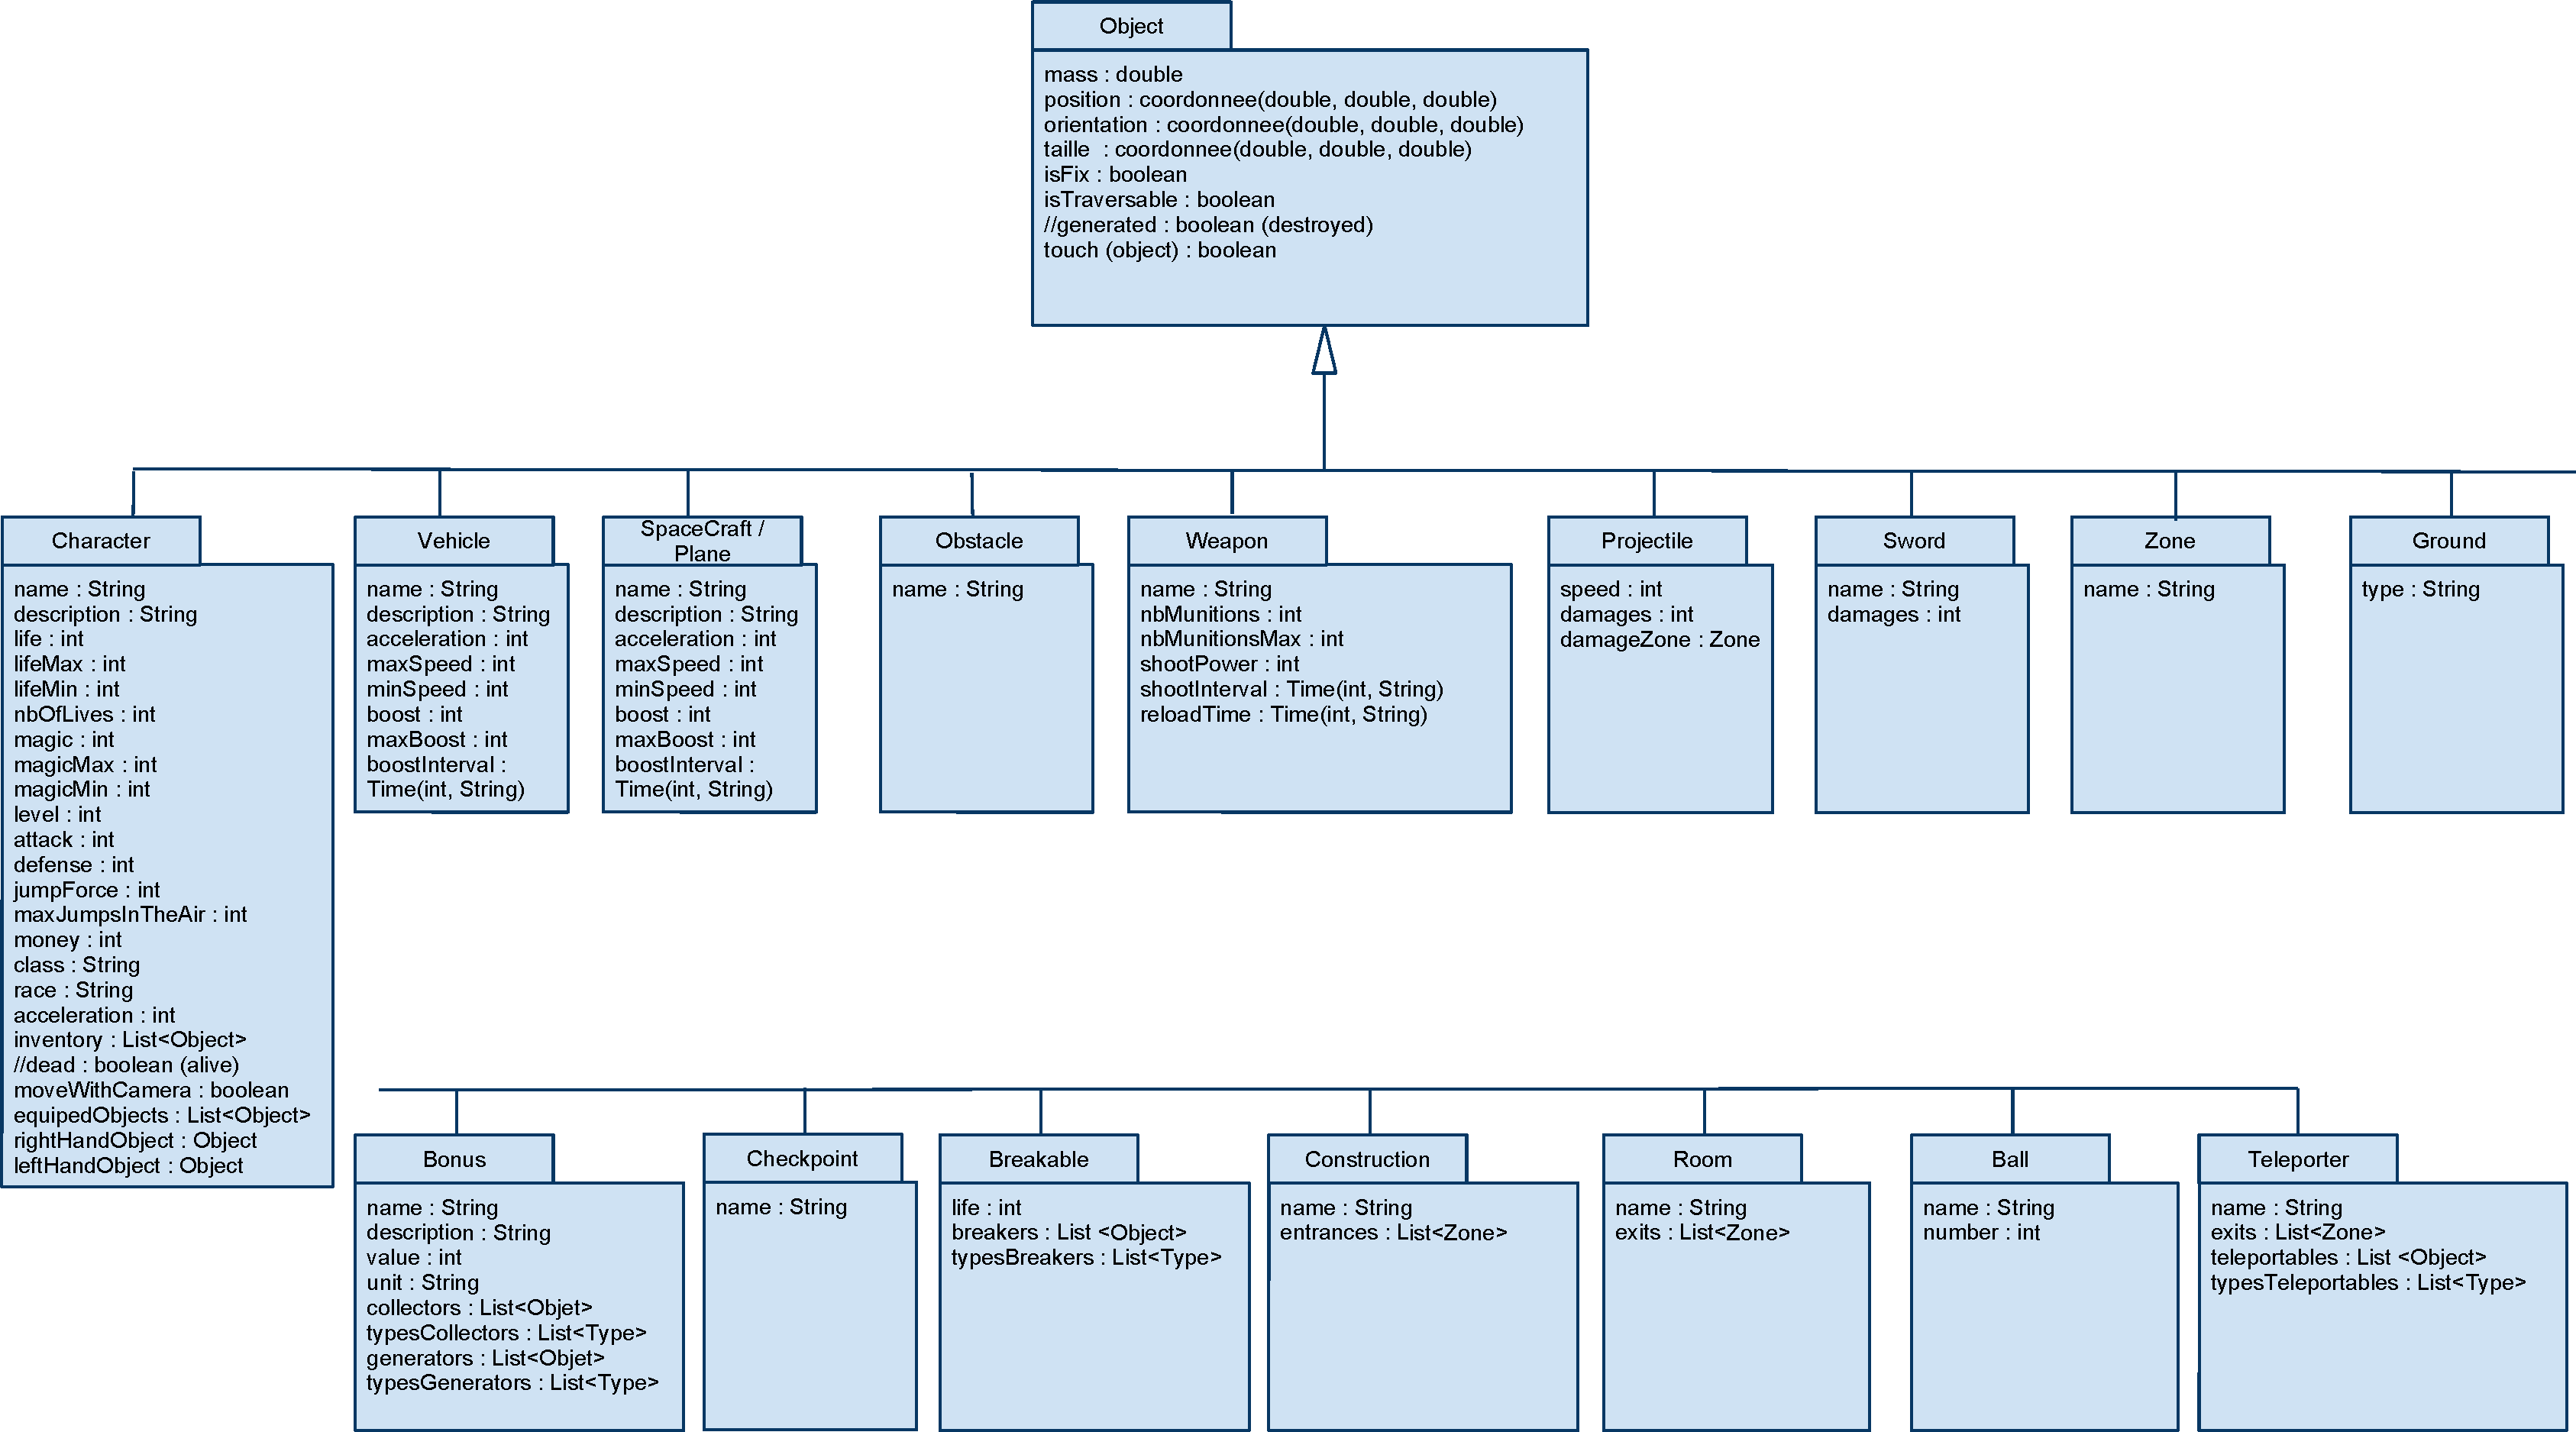
\includegraphics[width=\textwidth]{img/objectclass}
\end{figure}

Les divers attributs 'name' pourront servir lors de l'affichage d'information.
\code{gandalf is Character. gandalf has name at 'Gandalf le Blanc'.}

Les classes Character, Vehicle et Plane/SpaceCraft ont des comportements différents au niveau des commandes.

Pour un objet de type Character, le déplacement se fait directement lors de l'appui sur une touche. 
Il est possible d'initialiser l'attribut 'acceleration' pour avoir une physique plus réaliste comme Sonic ou Mario.
Un attribut 'moveWithCamera' permet d'indiquer si le personnage se déplace en fonction de la caméra courante. 
Par exemple, indiquer au personnage 'move backward' sans cet attribut le fera reculer.
Avec 'moveWithCamera', le personnage avancera vers la caméra.

Pour un ojet de type Vehicle, son délacement se fait uniquement avec son accélération et le fait de tourner dans une direction
 se fera uniquement si le véhicule n'est pas à l'arrêt.

Enfin pour un objet de type Plane, SpaceCraft, sa masse est nulle s'il avance, et tourner dans une direction signifie
effectuer une rotation suivant l'axe que forme sa trajectoire.

Pour les Obstacles, ils héritent des attributs isFix et isTraversable de Object et sont mis respectivement à true et false.

Concernant les Projectiles, ils se déplacent dès qu'ils sont générés et peuvent avoir une zone de dégâts dans le cas d'un missile par exemle.

Une Zone correspond à un volume englobant invisible et traversable par tous.

La classe Ground peut avoir plusieurs types comme la neige, qui a donc un coefficient de frottement faible, ou l'eau qui est traversable.

Un Bonus possède une liste d'objets ou de types d'objets qui peuvent le ramasser. Dès qu'une entité de ce type entre en contact avec le bonus, celui-ci
disparaît et a un effet sur elle. 
Il contient aussi une liste d'objets ou de types d'objets qui peuvent le générer lorsqu'ils disparaîssent.

Le Checkpoint est une Zone particulière : si le joueur meurt, il réapparaît à cet endroit. 
Le checkpoint peut aussi servir dans un jeu de course pour obliger le joueur à passer à cet endroit (exemple : TrackMania).

Les objets de la classe Breakable correspondent à un Object à 2 états, représenté par 2 fichiers 3D différents. Les deux états correspondent
à une vie nulle ou une vie strictement positive. Un exemple concret est une fenêtre. 
Dès qu'une balle (Projectile ayant un attribut 'damages') la traverse, elle passe dans l'état cassée avec la représentation 3D associée.

Une Construction correspond à une vue extérieure d'un bâtiment, d'une maison...
Ce type d'objet est associé à Room pour des jeux de rôles ou il n'est pas nécessaire de représenter une maison à sa taille réelle pour y entrer ensuite.
Une liste d'entrées correspond à des zones de téléporteurs associés aux sorties de Room le plus souvent.

Un objet de type Room reprend le principe de Construction mais les collisions sont gérées via des plans car un personnage à l'intérieur est considéré comme déjà en collision. 
Elle contient des sorties associées aux entrées d'une Construction ou d'une autre Room.

Un objet de type Ball a un volume englobant sphérique.

\subsection{Les autres classes}

Ci-dessous se trouvent les autres classes prédéfinies pour la grammaire haut-niveau.

\begin{figure}[h]
 \centering
 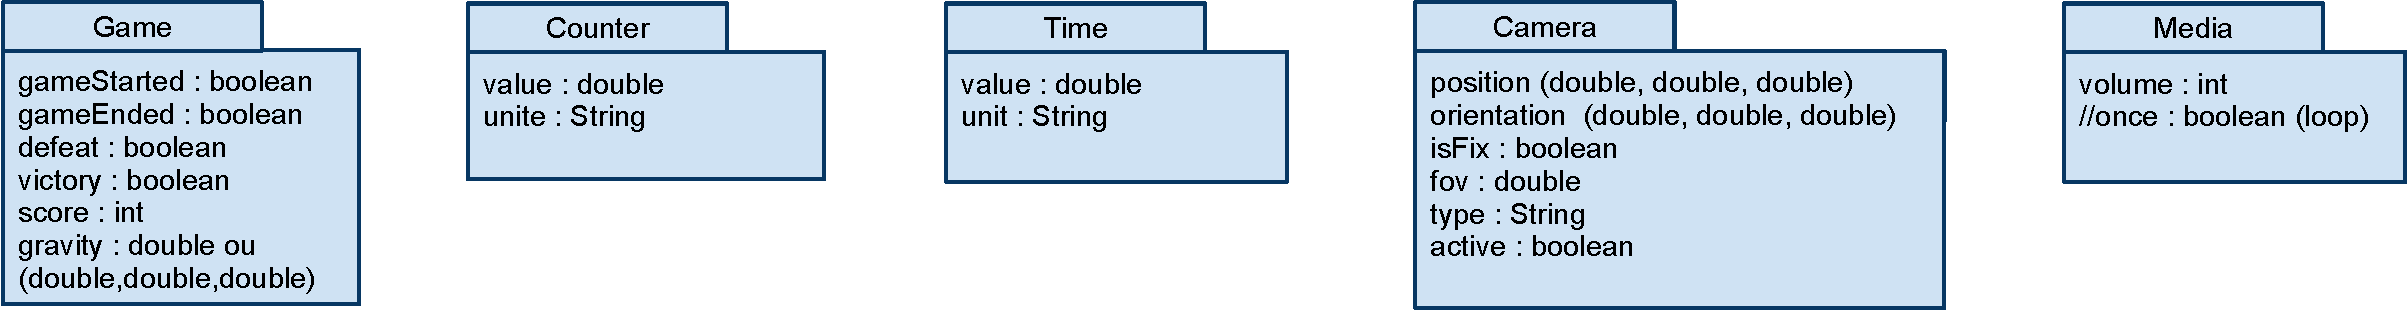
\includegraphics[width=\textwidth]{img/otherclass}
\end{figure}

La classe Game ne peut être instanciée qu'une seule fois.

Les ressources temporelles peuvent avoir plusieurs unités telles que les secondes, les millisecondes, les minutes ou les frames.

On peut définir la caméra selon un suivi à la première personne ('firstPerson') ou à la troisième personne ('thirdPerson') par rapport 
à l'objet qui aura été défini comme étant 'player'.
On peut aussi ne rien définir ou mettre 'free' pour une caméra libre.

Un Media a des mots-clefs dédiés comme play, mute on, mute off, pause ou stop.
On peut choisir entre un Media répété en boucle ('loop') ou lu une unique fois ('once').

\subsection{La grammaire}

L'intégralité de la gramaire haut-niveau est maintenant présenté.

\begin{lstlisting}[language=Grammar]

/*------------------------------------------------------------------
* PARSER RULES
*------------------------------------------------------------------*/
 
jeu :
  (infosJeu '.')?
  (nouveauType '.')*
  (init '.')+
  (definition '.')*
  (commande '.')*
  (reglesJeu '.')*
  (iaBasique '.')*;
 

///////////////////////////// ( informations about the game)  //////////////////////////////////

infosJeu :
  'Game' 'has' ('gravity' | 'score' /*| ...*/ ) 'at' (NUMBER | NUMBER NUMBER NUMBER)
  ;

 
//////////////////////////// ( Inheritance )  /////////////////////////////
 
nouveauType :
  'type' ident 'is' (ident | typeObjet) ('and' ident | typeObjet)* // to declare a new type
  ;            
  
// ident | typeObjet : if it is an ident, check that it is defined before by the user and that is an inherited Object.

 
//////////////////////////// ( Initializations )  /////////////////////////////

init :
  ident 'is' declarationObjet
  | accesClasse 'has' affectationObjet (',' affectationObjet)* // check the types and its attributes
  ;
 
declarationObjet :
  (ident | typeObjet3D) ('player' | interaction ('duplicable')? )?         // interaction is neutral by default
  | 'list' ('of' (operation)? (ident) ('with' (operation)? (ident))* )?  //operation if the object is duplicable
  | 'Camera' (('first' | 'third') 'person' | 'free')?
  | 'Media' ('loop' | 'once')? 						 // sound, music or video played in loop or once
  | 'in' ident 				                         // ident of a list to add an element
;           
 
interaction :
  'ally' | 'enemy' | 'neutral'
  ;
 
affectationObjet :
  ident ('at' (operation (uniteTps)? | ident) )?       //aggregation
  | attribut 'at' (operation | STRING | BOOL)          //life at 5, name at "Gandalf Le Gris"
  | typeCoordonnees 'at' coordonnees            //size at 20 30 40
  | attributListeOuObjet 'at' ident             //inventory at listeArmesJoueur
  | attributTps 'at' operation uniteTps         //
  ;
 
// has ident at ... : to declare a new attribute
// Attributes of predefined class have default initialized
// it is not necessary to initialize not used attribute
  
typeObjet :
  'Camera'
  | 'Media'
  | 'Counter'
  | 'Time'
  | typeObjet3D
  ;
 
// every predefined classes
typeObjet3D:
  'Object'                      // -> position(x,y,z), orientation(x,y,z), size(x,y,z)
  | 'Character'                 // -> life, lifeMax, magic, magicMax , level, experience, attack, defense
  | 'Vehicle'                   // -> acceleration, speedMax,
  | 'Plane' | 'SpaceCraft'
  | 'Obstacle'                  // a fixed entity, used for collisions
  | 'Weapon'                    // -> nbMunitions, nbMaxMunitions, intervalleTirs, timeRecharge
  | 'Sword'                     // -> damages, level
  | 'Projectile'                // -> vitesse, damages, level(pourquoi pas)
  | 'Zone'                      // an invisible and traversable entity
  | 'Ground'                    // -> type of ground (water, snow ...)
  | 'Bonus'                     // an object which disappears when something touches it-> valeur(entier), nomObjet(type),listeObjets 
  | 'CheckPoint'
  | 'Breakable'
  | 'Construction'
  | 'Room'
  | 'Ball'
  | 'Teleporter'
  ;
 
// every attributes of predefined classes
attribut : 
  'mass'                  // attributes of object :
  | 'isFix'
  | 'isTraversable'
  | 'fov'                    // attributes of "camera"
  | 'type'
  | 'active'
  | 'name'                   // attributes of "character" :
  | 'description'
  | 'life'
  | 'lifeMax'
  | 'lifeMin'   
  | 'nbOfLives'   
  | 'magic'
  | 'magicMax'
  | 'magicMin'
  | 'level'
  | 'attack'
  | 'defense'
  | 'jumpForce'
  | 'maxJumpsInTheAir'
  | 'money'
  | 'class'
  | 'race'
  | 'acceleration'    
  | 'speed'                // attributes of "vehicle" :
  | 'maxSpeed'
  | 'minSpeed'
  | 'boost'
  | 'maxBoost'
  | 'nbMunitions'           // attributes of"weapon" :
  | 'nbMunitionsMax'        
  | 'shootPower'
  | 'damages'               //attributes of "projectile"
  | 'value'                // attributes of "bonus" :
  | 'unit'
  | 'objectname'
  | 'attributName'               
  | 'volume'                 //attributes of "media"
  | 'number'              //attributes of "ball"
  | 'moveWithCamera'
  ;
 
attributListeOuObjet :
  'inventory'
  | 'equipedObjects'
  | 'entrances'
  | 'exits'
  | 'damageZone'
  | 'collectors'
  | 'typesCollectors'
  | 'generators'
  | 'typeGenerators'
  | 'breakers'
  | 'typesBreakers'
  | 'teleportables'
  | 'typesTeleportables'
  ;
 
attributTps :
  'boostInterval'
  | 'shootInterval'        //attributes of "weapon" :
  | 'reloadTime'
  ;
 

//////////////////////////// ( new definitions of actions ) ///////////////////
 
definition : 'definition' ident 'means' consequences;
 
consequences :
  consequ (',' consequ)*
  ;
  
consequ :
  siAlors
  | action
  | affectation
  | activCommande
  | appelDef
  | 'victory'
  | 'defeat'
  ;
 
appelDef :
  ident           //ident of a definition of an action (means)
  ;
 
activCommande :
  ('activate' | 'disable') ('commands' | 'mouse' (souris (',' souris)*)? | 'key' clavier (',' clavier)* | 'keyboard' )
  ;
//disable commands              // all the commands
//disable key                   // all the key commands
//disable mouse up, down        // only move up or down with the mouse
 

//////////////////////////// ( Initialization of commands )  /////////////////////////////

commande :
  'command' (ident 'is' actionCommande (',' actionCommande)* | actionCommande)
  ;

actionCommande :
  ('mouse' souris | 'key' clavier) 'for' (ident | actionCommandePressee | actionCommandeMaintenue) // ident : what is defined with means
  ;
 
souris :
        'up' | 'down' | 'left' | 'right' | 'lClick' | 'cClick' | 'rClick' | 'scrollUp' | 'scrollDown'
        ;
 
clavier :
        CHAR | 'up' | 'down' | 'left' | 'right' | 'space' | 'echap' | 'enter'          //CHAR : Z,Q,S,D,...
        ;
 
actionCommandePressee :
  'jump' operation
  | 'pause'
  | 'stop'
  ;
actionCommandeMaintenue :
  'move' ('left' | 'right' | 'forward' | 'backward')
  | 'turn' ('left' | 'right')
  | 'accelerate'
  | 'brake'
  ;
 
 
//////////////////////////// ( Rules of the game + conditions of victory / defeat )  /////////////////////////////

reglesJeu :
  'rule' (ident 'is')? declencheur 'then' consequences ','
  ;
conditions :
  conditionEt ('or' conditionEt)*
  ;
 
conditionEt :
  conditionsNot ('and' conditionsNot)*
  ;
  
conditionsNot :
  'not' cond
  ;

cond :
  '(' conditions ')'
  | etat
  | operation comparaison operation
  ;

etat :
  accesClasse 'is' ('not')? ('dead' | 'alive' | 'effaced' | 'generated' | 'touching' (('other')? accesGlobal | accesLocal))  // for an object
  | (ident | 'game') 'is' ('not')? ('finished' |'started' | 'paused' | 'muted' ('on' | 'off') | 'played' | 'stopped' )  // game,counter,media
  | 'true'                                                   
  | 'victory'
  | 'defeat'
  ;
 
declencheur :
  accesClasse ('dies' | ('touches' | 'kills') (('other')? accesGlobal | accesLocal) | ('killed' | 'touched') ('by' (('other')? accesGlobal | accesLocal))? )
  | (ident | 'game') ('ends' |'starts')          //ident if it is a counter
  | variable 'becomes' varOuNb
  | ident 'becomes' ('player' | interaction)
  ;
  
siAlors :
  'if' conditions 'then' consequences ('else' consequences)? 'end'
  ;
  
 
action :
  accesClasse actionObjet
  | (ident | 'game') ('ends' |'starts')
  | ('pause' | 'mute' ('on' | 'off') | 'play' | 'stop' ) ident
  | 'block' transformation 'of' accesClasse coordonnees
  | ('efface' | 'generate') (accesClasse | operation accesClasse ('in' accesLocal | 'on' accesLocal | 'at' coordonnees)?)
  | 'wait' operation uniteTps 'then' consequences 'endWait'
  | 'save'
  ;
 
actionObjet :
  'dies'
  | actionCommandePressee
  | actionCommandeMaintenue ('during' operation uniteTps | 'until' conditions)
  | 'equip' (accesLocal | 'next' | 'previous')   
  ;
 
affectation :
  (('assign' | 'add' | 'sub') operation) 'for' variable | 'invert' variable 'with' variable
  ;

//add : a += b, remove : a -= b, assign : a = b, invert : tmp=a; a=b; b=tmp;

coordonnees :
  operation operation operation
  ;
 
comparaison :
  '=' | '<' | '>' | '<=' | '>='
  ; 
 
transformation :
  'translation'
  | 'rotation'
  | 'scale'
  ;
 
uniteTps :
  'mn'
  | 'sec'
  | 'ms'
  | 'frames'
  ;
 
operation :
  ('random' 'between' operationPlus 'and')? operationPlus
  ;
 
operationPlus :
  operationMul (operateurPlus operationMul)*
  ;
operationMul :
  operationPuiss (operateurMul operationPuiss)*
  ;
  
operationPuiss :
  operationparentheses ('^' operationparentheses)*
  ;
  
operationparentheses :
  '(' operation ')'
  | varOuNb
  ;
 
varOuNb :
  variable
  | NUMBER
  ;
 
variable :
  (('x' | 'y' | 'z') 'of' (typeCoordonnees | ident | attribut)) 'of' accesClasse
                      //x of size of num 10 in listeWeapon
  ;
 
accesClasse : accesLocal | accesGlobal;
 
accesGlobal :
  typeObjet
  | interaction
  | 'not' (typeObjet | interaction | 'player')
  | 'all'
  ;
 
accesLocal :
  ident
  | 'num' operation 'in' ident
  | 'player'
  ;
 
 
typeCoordonnees :
  'positition' | 'rotation' | 'scale'
  ;
 
operateur :
  operateurMul
  | operateurPlus
  ;
  
operateurMul :
  '*'
  | '/'
  | '%'
  ;
  
operateurPlus :
  '+'
  | '-'
  ;
 
ident :
  STRING
  ;
 
//////////////////////////// ia //////////////////////////
 
iaBasique : 'ia' accesClasse 'is' actionObjet (',' actionObjet)*;
 

/*------------------------------------------------------------------
* LEXER RULES
*------------------------------------------------------------------*/
BOOL        : ('true' | 'false');
STRING        :  ('a'..'z' | 'A'..'Z') ('a'..'z' | 'A'..'Z' | '0'..'9')+ ;
CHAR   : 'a'..'z' | 'A'..'Z';
NUMBER : ('0'..'9')+ (',' ('0'..'9')+ )? ;
WS  :   ( ' '  
           | '\t'  
           | '\r'  
           | '\n'  
           | '\u000C'
           )+ {$channel=HIDDEN;}  
        ;
\end{lstlisting}
